% questions.tex -- Module 8 (From the Universe to the Atom) short-answer booklet, HSC Section II style.
% 20 questions, 90 marks, 18 marks per topic: Topic 1 Q1-4, Topic 2 Q5-8, Topic 3 Q9-12,
% Marking guidelines and sample answers: answers.tex.
% Every number (and the Q14 curve): checks/m8-short-answer/numbers.py
% Build: TEXINPUTS=.: xelatex questions.tex (twice)
\documentclass[12pt]{article}
\usepackage{mathtools}
\usepackage{quiz}
\hypersetup{pdftitle={Short Answer Questions - Module 8 - From the Universe to the Atom}}
\newcommand\nuc[3]{\ensuremath{\prescript{#1}{#2}{\mathrm{#3}}}}

\begin{document}
\quiztitle{Year 12 Physics}{Short Answer Questions - Module 8 - From the Universe to the Atom}
\begin{center}
  20 questions \textperiodcentered\ 90 marks \textperiodcentered\ allow about 2 hours 40 minutes\\[2pt]
  Show all working. Use $c = \qty{3.00e8}{m.s^{-1}}$, $h = \qty{6.626e-34}{J.s}$,
  $e = \qty{1.602e-19}{C}$, $m_\mathrm{e} = \qty{9.109e-31}{kg}$, $m_\mathrm{p} = \qty{1.673e-27}{kg}$,\\
  $\qty{1}{u} = \qty{1.661e-27}{kg} = \qty{931.5}{MeV}/c^2$, $R = \qty{1.097e7}{m^{-1}}$,
  $g = \qty{9.8}{m.s^{-2}}$, $\qty{1}{eV} = \qty{1.602e-19}{J}$.
\end{center}

% =====================================================================
\firsttopictitle{Topic 1 - Origins of the Elements}

% ---- Q1 (Hubble's law and the age of the universe)
\begin{saq}{5}
The graph shows the recession velocities and distances of five galaxies, with a line of best fit.
\begin{center}
  \begin{tikzpicture}[x=0.06cm, y=0.0006cm]
    \draw[black!20, line width=0.3pt, xstep=10, ystep=500] (0,0) grid (100,7000);
    \draw[axisline] (0,0) -- (108,0) node[right, font=\small] {$d$ (Mpc)};
    \draw[axisline] (0,0) -- (0,7600) node[above, font=\small] {$v$ (\si{km.s^{-1}})};
    \foreach \x in {0,20,...,100} \node[below, font=\scriptsize] at (\x,0) {\x};
    \foreach \y in {1000,2000,...,7000} \node[left, font=\scriptsize] at (0,\y) {\y};
    \draw[line width=1pt] (0,0) -- (100,6800);
    \foreach \x/\y in {20/1300, 40/2800, 60/4000, 80/5500, 100/6800} \fill (\x,\y) circle (2.2pt);
  \end{tikzpicture}
\end{center}
\qpartL{a}{2}{Use the graph to determine the Hubble constant, in \si{km.s^{-1}.Mpc^{-1}}.}{4}
\qpartL{b}{2}{Estimate the age of the universe, in years, using $t = \dfrac{1}{H_0}$.
($\qty{1}{Mpc} = \qty{3.09e22}{m}$, $\qty{1}{year} = \qty{3.16e7}{s}$)}{4}
\qpartL{c}{1}{Explain how Hubble's observations support the Big Bang theory.}{2}
\end{saq}

% ---- Q2 (energy into matter after the Big Bang)
\Needspace{140mm}
\begin{saq}{4}
Describe how the matter in the universe formed from energy in the time after the Big Bang, up to the
formation of the first neutral atoms.
\alines{11}
\end{saq}

% ---- Q3 (HR diagram)
% P lower left (white dwarf), Q upper right (red giant), R middle of main sequence (Sun), S upper left (massive)
\Needspace{50\baselineskip}
\begin{saq}{5}
The Hertzsprung--Russell diagram shows four stars, P, Q, R and S. Star R is the Sun.
\begin{center}
  \begin{tikzpicture}[x=1cm, y=0.5cm]
    \draw[line width=0.7pt] (0,0) -- (6.4,0) node[right, font=\small, align=left] {Surface\\temperature};
    \draw[axisline] (0,0) -- (0,8.6) node[above, font=\small] {Luminosity (Sun $= 1$)};
    \foreach \y/\l in {1/$10^{-4}$, 3/$10^{-2}$, 5/$1$, 7/$10^{2}$} {\draw (0,\y) -- (-0.08,\y) node[left, font=\scriptsize] {\l};}
    \foreach \x/\l in {0.5/\qty{30000}{K}, 3/\qty{10000}{K}, 5.5/\qty{3000}{K}} {\draw (\x,0) -- (\x,-0.15) node[below, font=\scriptsize] {\l};}
    \draw[line width=6pt, black!15, line cap=round, smooth] plot coordinates {(0.6,8.4) (2.0,7.6) (3.2,6.5) (4.16,5.0) (4.9,3.4) (5.6,1.6)};
    \fill (1.3,3.0) circle (2.5pt) node[right, font=\small] {P};
    \fill (5.1,7.0) circle (2.5pt) node[right, font=\small] {Q};
    \fill (4.16,5.0) circle (2.5pt) node[right, font=\small] {R};
    \fill (0.9,8.25) circle (2.5pt) node[right, font=\small] {S};
  \end{tikzpicture}
\end{center}
\qpartL{a}{1}{Which main-sequence star has the greatest mass? Justify your answer.}{2}
\qpartL{b}{2}{Compare the surface temperatures and radii of stars P and Q.}{4}
\qpartL{c}{2}{Describe how the Sun's position on the diagram will change as it evolves after it leaves
the main sequence.}{4}
\end{saq}

% ---- Q4 (energy from fusion; p-p chain and CNO cycle)
\Needspace{36\baselineskip}
\begin{saq}{4}
In the core of a star, hydrogen is fused into helium. The overall result can be written as four hydrogen
atoms (\qty{1.007825}{u} each) forming one helium-4 atom (\qty{4.002603}{u}).
\qpartL{a}{2}{Calculate the energy released, in MeV, for each helium-4 atom formed.}{4}
\qpartL{b}{2}{Compare the proton--proton chain and the CNO cycle.}{4}
\end{saq}

% =====================================================================
\topictitle{Topic 2 - Structure of the Atom}

% ---- Q5 (Thomson's charge-to-mass ratio)
\begin{saq}{5}
In an experiment like Thomson's, cathode rays pass between parallel plates \qty{2.0}{cm} apart with a
potential difference of \qty{400}{V}. A magnetic field of \qty{8.0e-4}{T} at right angles to the electric
field is adjusted so that the beam passes straight through.
\qpartL{a}{2}{Calculate the speed of the cathode rays.}{4}
\qpartL{b}{2}{The electric field is switched off, and the beam moves in a circular arc of radius
\qty{0.18}{m}. Calculate the charge-to-mass ratio of the cathode-ray particles.}{4}
\qpartL{c}{1}{The charge-to-mass ratio of a hydrogen ion is \qty{9.6e7}{C.kg^{-1}}. What did Thomson
conclude from comparing this with his result?}{2}
\end{saq}

% ---- Q6 (Millikan)
\Needspace{30\baselineskip}
\begin{saq}{4}
In a Millikan oil-drop experiment, an oil drop of mass \qty{3.27e-15}{kg} is held stationary in a uniform
electric field of \qty{4.0e4}{V.m^{-1}}, directed downwards.
\qpartL{a}{2}{Calculate the charge on the drop, and state its sign.}{4}
\qpartL{b}{1}{How many excess electrons does the drop carry?}{2}
\qpartL{c}{1}{How did Millikan's results show that electric charge is quantised?}{2}
\end{saq}

% ---- Q7 (Geiger-Marsden and Rutherford)
\Needspace{150mm}
\begin{saq}{5}
Describe the Geiger--Marsden experiment, and explain how its results led Rutherford to a new model of the
atom.
\alines{13}
\end{saq}

% ---- Q8 (Chadwick)
\Needspace{130mm}
\begin{saq}{4}
The diagram shows a simplified version of Chadwick's experiment.
\begin{center}
  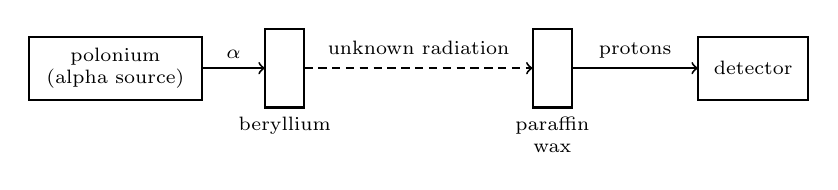
\begin{tikzpicture}
    \draw[line width=0.8pt] (0,0) rectangle (2.2,0.8); \node[font=\scriptsize, align=center] at (1.1,0.4) {polonium\\(alpha source)};
    \draw[->, line width=0.7pt] (2.2,0.4) -- (3.0,0.4); \node[above, font=\scriptsize] at (2.6,0.4) {$\alpha$};
    \draw[line width=0.8pt] (3.0,-0.1) rectangle (3.5,0.9); \node[below, font=\scriptsize] at (3.25,-0.1) {beryllium};
    \draw[->, line width=0.7pt, dash pattern=on 3pt off 2pt] (3.5,0.4) -- (6.4,0.4); \node[above, font=\scriptsize] at (4.95,0.45) {unknown radiation};
    \draw[line width=0.8pt] (6.4,-0.1) rectangle (6.9,0.9); \node[below, font=\scriptsize, align=center] at (6.65,-0.1) {paraffin\\wax};
    \draw[->, line width=0.7pt] (6.9,0.4) -- (8.5,0.4); \node[above, font=\scriptsize] at (7.7,0.4) {protons};
    \draw[line width=0.8pt] (8.5,0) rectangle (9.9,0.8); \node[font=\scriptsize] at (9.2,0.4) {detector};
  \end{tikzpicture}
\end{center}
Explain how this experiment provided evidence for the existence of the neutron.
\alines{10}
\end{saq}

% =====================================================================
\topictitle{Topic 3 - Quantum Mechanical Nature of the Atom}

% ---- Q9 (hydrogen spectrum)
\begin{saq}{5}
The diagram shows some of the energy levels of the hydrogen atom (not to scale).
\begin{center}
  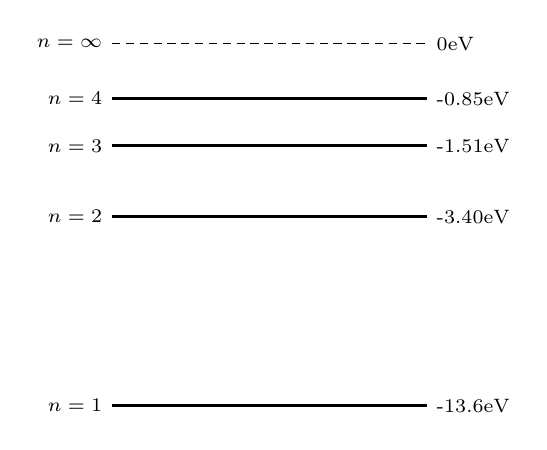
\begin{tikzpicture}
    \foreach \n/\E/\y in {1/-13.6/0, 2/-3.40/2.4, 3/-1.51/3.3, 4/-0.85/3.9} {
      \draw[line width=1pt] (0,\y) -- (4,\y);
      \node[left, font=\scriptsize] at (0,\y) {$n = \n$};
      \node[right, font=\scriptsize] at (4,\y) {\qty{\E}{eV}};}
    \draw[line width=0.6pt, dash pattern=on 3pt off 2pt] (0,4.6) -- (4,4.6);
    \node[left, font=\scriptsize] at (0,4.6) {$n = \infty$}; \node[right, font=\scriptsize] at (4,4.6) {\qty{0}{eV}};
  \end{tikzpicture}
\end{center}
\qpartL{a}{2}{Use the Rydberg equation to calculate the wavelength of the light emitted when an electron
moves from $n = 4$ to $n = 2$.}{4}
\qpartL{b}{2}{Show that the energy of this photon agrees with the energy-level diagram.}{4}
\qpartL{c}{1}{In which part of the electromagnetic spectrum is this light?}{1}
\end{saq}

% ---- Q10 (assessing Bohr's model)
\Needspace{130mm}
\begin{saq}{4}
Assess the contribution of Bohr's model to our understanding of the atom.
\alines{12}
\end{saq}

% ---- Q11 (electron diffraction)
\Needspace{34\baselineskip}
\begin{saq}{5}
Electrons are accelerated from rest through a potential difference of \qty{150}{V}.
\qpartL{a}{2}{Calculate the speed of the electrons.}{4}
\qpartL{b}{2}{Calculate the de Broglie wavelength of the electrons.}{3}
\qpartL{c}{1}{Explain why these electrons can be diffracted by a crystal.}{2}
\end{saq}

% ---- Q12 (de Broglie and Bohr; evidence)
\Needspace{125mm}
\begin{saq}{4}
Explain how de Broglie's matter-wave hypothesis accounted for Bohr's stationary states, and outline ONE
piece of experimental evidence for matter waves.
\alines{11}
\end{saq}

% =====================================================================
\topictitle{Topic 4 - Properties of the Nucleus}

% ---- Q13 (activity graph)
\begin{saq}{5}
The graph shows the measured activity of a radioactive sample over 24 days, with a smooth curve of best
fit.
\begin{center}
  \begin{tikzpicture}[x=0.27cm, y=0.0032cm]
    \draw[black!20, line width=0.3pt, xstep=3, ystep=100] (0,0) grid (24,1200);
    \draw[axisline] (0,0) -- (26,0) node[right, font=\small] {Time (days)};
    \draw[axisline] (0,0) -- (0,1330) node[above, font=\small] {Activity (Bq)};
    \foreach \x in {0,6,...,24} \node[below, font=\scriptsize] at (\x,0) {\x};
    \foreach \y in {200,400,...,1200} \node[left, font=\scriptsize] at (0,\y) {\y};
    \draw[line width=1pt, domain=0:24, samples=60, smooth] plot (\x, {1200*2^(-\x/6)});
    \foreach \x/\y in {0/1200, 3/860, 6/590, 9/430, 12/295, 15/215, 18/148, 21/108, 24/74} \fill (\x,\y) circle (2.2pt);
  \end{tikzpicture}
\end{center}
\qpartL{a}{1}{Use the graph to determine the half-life of the sample.}{2}
\qpartL{b}{1}{Calculate the decay constant.}{2}
\qpartL{c}{2}{Calculate the activity of the sample after 40 days.}{4}
\qpartL{d}{1}{Explain why the measured points do not lie exactly on the curve.}{2}
\end{saq}

% ---- Q14 (binding energy per nucleon)
\Needspace{48\baselineskip}
\begin{saq}{4}
The graph shows the binding energy per nucleon of nuclei against their mass number $A$.
\begin{center}
  \begin{tikzpicture}[x=1cm, y=0.45cm]
    \draw[axisline] (0,0) -- (6.5,0) node[right, font=\small] {$A$};
    \draw[axisline] (0,0) -- (0,10) node[above, font=\small] {Binding energy per nucleon (MeV)};
    \foreach \x/\l in {0/0, 1.25/50, 2.5/100, 3.75/150, 5/200, 6.25/250} \draw (\x,0) -- (\x,-0.15) node[below, font=\scriptsize] {\l};
    \foreach \y in {2,4,6,8} \draw (0,\y) -- (-0.08,\y) node[left, font=\scriptsize] {\y};
    \draw[line width=1pt, smooth] plot coordinates {(0.050,1.11) (0.075,2.57) (0.150,5.33) (0.175,5.61) (0.225,6.46) (0.300,7.68) (0.400,7.98) (0.500,8.03) (0.750,8.52) (1.000,8.55) (1.400,8.79) (2.000,8.69) (2.500,8.60) (3.000,8.50) (3.750,8.27) (4.500,8.05) (5.250,7.83) (5.950,7.57)};
    \fill (0.1,7.07) circle (2pt); \draw[line width=0.4pt] (0.13,6.95) -- (0.6,5.4) node[right, font=\scriptsize] {\nuc{4}{2}{He}};
    \fill (1.4,8.79) circle (2pt) node[above, font=\scriptsize] {\nuc{56}{26}{Fe}};
    \fill (5.95,7.57) circle (2pt) node[above, font=\scriptsize] {\nuc{238}{92}{U}};
  \end{tikzpicture}
\end{center}
Use the graph to explain why energy is released both when heavy nuclei undergo fission and when light
nuclei undergo fusion.
\alines{9}
\end{saq}

% ---- Q15 (fission energy)
\Needspace{40\baselineskip}
\begin{saq}{5}
A uranium-235 nucleus absorbs a neutron and undergoes fission:
\[ \nuc{235}{92}{U} + \nuc{1}{0}{n} \rightarrow \nuc{141}{56}{Ba} + \nuc{92}{36}{Kr} + x\,\nuc{1}{0}{n} \]
The masses are: \nuc{235}{92}{U} \qty{235.0439}{u}; \nuc{141}{56}{Ba} \qty{140.9144}{u}; \nuc{92}{36}{Kr}
\qty{91.9262}{u}; \nuc{1}{0}{n} \qty{1.008665}{u}.
\qpartL{a}{1}{Determine the value of $x$.}{2}
\qpartL{b}{2}{Calculate the energy released in one fission, in MeV.}{4}
\qpartL{c}{2}{Calculate the energy released when \qty{1.0}{kg} of uranium-235 undergoes fission in this
way.}{4}
\end{saq}

% ---- Q16 (alpha, beta, gamma)
\Needspace{120mm}
\begin{saq}{4}
Compare alpha, beta-minus and gamma radiation in terms of their nature, charge and penetrating ability,
and explain how a magnetic field could be used to tell them apart.
\alines{11}
\end{saq}

% =====================================================================
\topictitle{Topic 5 - Deep Inside the Atom}

% ---- Q17 (Standard Model classification)
\begin{saq}{4}
\qpartL{a}{1}{A proton is made of two up quarks ($+\frac{2}{3}e$ each) and one down quark
($-\frac{1}{3}e$). Show that its charge is $+e$.}{2}
\qpartL{b}{1}{A positive pion ($\pi^+$) is made of an up quark and an anti-down quark. What is its
charge?}{2}
\qpartL{c}{2}{Classify each of these particles as a lepton, baryon, meson or gauge boson: electron,
neutron, $\pi^+$, photon.}{3}
\end{saq}

% ---- Q18 (beta decay and the neutrino)
\Needspace{150mm}
\begin{saq}{5}
In beta-minus decay, the emitted electrons have a range of kinetic energies, from zero up to a maximum
value. Explain how this observation led to the prediction of the neutrino, and describe beta-minus decay at
the quark level.
\alines{13}
\end{saq}

% ---- Q19 (Large Hadron Collider)
\Needspace{34\baselineskip}
\begin{saq}{5}
Since 2022, the Large Hadron Collider has accelerated protons to a total energy of \qty{6.8}{TeV}
($\qty{6.8e12}{eV}$).
\qpartL{a}{2}{Calculate the Lorentz factor $\gamma$ of these protons, using $E = \gamma mc^2$.}{4}
\qpartL{b}{2}{Explain why such high energies are needed to discover new particles.}{4}
\qpartL{c}{1}{Explain why the speed of these protons is very close to, but less than, the speed of
light.}{2}
\end{saq}

% ---- Q20 (protons are not fundamental)
\Needspace{125mm}
\begin{saq}{4}
Analyse the evidence that protons and neutrons are not fundamental particles.
\alines{11}
\end{saq}

\end{document}
